\chapter{Backend Mystery} 
Teakwood is powered by Django framework, so its backend inherits all the Django  backend feathers. For example, Teakwood follows the MVC(Model-View-Controller) design pattern and DRY(Don't Repeat Yourself) principle. When you go through Teakwood's code, you will find that teakwood have a neat and loose coupling coding structure. What makes Teakwood's coding structure so unique? This chapter will go through Teakwood's four important feathers in the backend: The MTV design pattern, the model to database mapping, the template language and the powerfull admin system.

\section{MTV Framework}
Teakwood has an updated MVC, that is MTV.\\
\begin{figure}[htb]
\centering
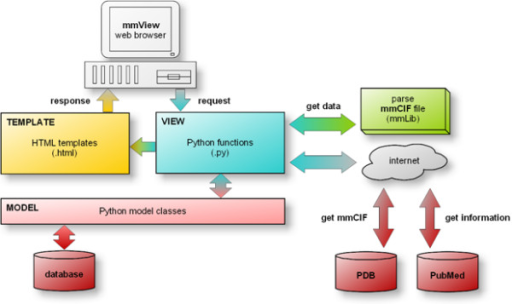
\includegraphics[scale=0.7]{./mtv}
\caption{Teakwood MTV framework}
\label{fig:label} % insert suitable label, this is used to refer to a fig from within the text as shown above
\end{figure}

\textbf{M} represents the model (Model), i.e., \textbf{the data access layer}. This layer processing data in all matters related to: how to access, how to confirm the validity , which behaviors it has, and the relationships between the data.\\
\textbf{T} Represents the template (Template), i.e., \textbf{the presentation layer}. This layer response for how to display the page or other types of documents.\\
\textbf{V} represents the view (View), \textbf{business logic layer}. You can see it as a bridge between the model and the template.This layer calls the model to provide data and sent it template for rendering web page. \\
\vspace{1in}

As we can see from the figure, Teakwood has a loose coupled modeling design. "M","T", and "V" are separated from each other; Each MTV wrapper(i.e. a Django app) is also separated from each other. This design makes the Teakwood sytem flexible for making changes and easy to extend feathers.

\section{Models and Database}
Teakwood provides an abstraction layer (the “models”) for structuring and manipulating the data of Teakwood apps. Essentially, a model is a Python object that describes your data model/table.Thanks for Django's integrated object relational mapping (ORM) functions, we don't have work with SQL database in order to manipulate data, all we should do is manipulating the corresponding Python object. ORM will do the mapping work.

Django provides many APIs to deal with Databases by invoking corespondent python object.

\section{Teakwood Template Language}
Teakwood’s template language is designed to strike a balance between power and ease. Its designed to please both the HTML designer and the Python coder. \\
Teakwood template language is not just HTML file or Python code. Here is an example:
\begin{verbatim}

{{ section.title }}

<h1>{{ section.title }}</h1>

<h2><a href="{{ story.get_absolute_url }}">
    {{ story.headline|upper }}
  </a></h2>
<p>{{ story.tease|truncatewords:"100" }}</p>


\end{verbatim}

We can see there are some special symbols in the HTML code. In Django template language they are called variables, tags and filters.\\

\textbf{Variable}: When the template engine encounters a variable, it evaluates that variable and replaces it with the result.\\
\textbf{Tag }: Tags are more complex than variables: Some create text in the output, some control flow by performing loops or logic, and some load external information into the template to be used by later variables. Some tags require beginning and ending tags. \\
\textbf{filter}:Filter is basically a restricted variable.\\

Through variables and tags, static HTML files becomes dynamic HTML files and can interact with python code. Django system even provides build-in tags for achieving the logical control.


\section{Powerful Admin}
Teakwood comes with a user authentication system which is inherited from Django framework also. The admin system handles user accounts, groups, permissions and cookie-based user sessions. 

Teakwood Admin system limited to trusted site administrators, that enables the adding, editing and deletion of site content. Some common examples: the interface you use to post to your blog, the backend site managers use to moderate user-generated comments, the tool your clients use to update the press releases on the Web site you built for them. All these cases can be handled in Admin console.

\section{A Practical Case}

So far we've already know that Teakwood is loose coupling designed and follows a "MTV"design pattern; we also know that Teakwood uses python object to work with database by object oriented mapping; plus, Teakwood template language is powerful for generating HTML files, now let's connect all these details to see How Teakwood process a request from user. 
Fisrt, let's take a look at the Teakwood HTTP request response flow.\\

\begin{figure}[h]
\centering
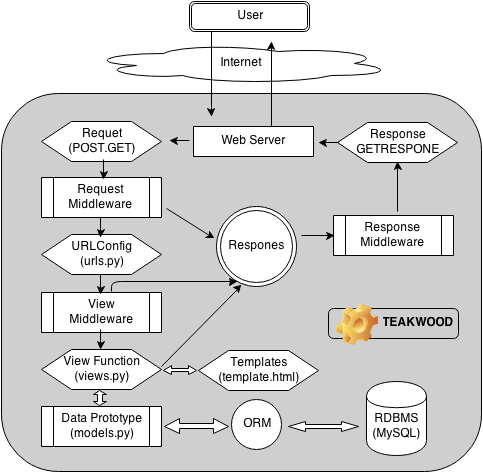
\includegraphics[scale=0.4]{./http_request_response}
\caption{Teakwood Request-Response Working Flow}
\label{fig:label} % insert suitable label, this is used to refer to a fig from within the text as shown above
\end{figure}
Now let take a real example to see how this structure works. For example, an user want to view all the job status under his/her account.
$\bullet$ Click the job button.\\
$\bullet$ Button triggered an request.\\
$\bullet$ Request goes to request middleware for identity check, if legal? auth?\\
$\bullet$ if yes, goes to response and raise error page;\\
$\bullet$ if no, goes to urlconfig to locate the right URL.\\
$\bullet$ URL goes to view middleware for legibility check, if wrong URL, auth?\\
$\bullet$ if yes, goes to response and raise an error page;\\
$\bullet$ if no, goes to view function. \\
$\bullet$ View function check if need data? if need template?\\
$\bullet$ if need data, trigger models to fetch data from database;\\
$\bullet$ if need template, find the right template, also fetch css, js and imgs.\\
$\bullet$ Send all files to response and rendering web page.\\
$\bullet$ Display the final page to user.



%\section{Lose Coupling}


